\section{Semantic-Lifting}
\label{sec:lifting}

Als Eingabe für das Semantic-Lifting dient die zuvor berechnete technische Differenz der Modelle A
und B. Die technische Differenz enthält ausschließlich low-level Änderungen, welche angeben, was
sich zwischen Modell A und Modell B verändert hat. Da low-level Änderungen auf Basis des Metamodells
angegeben werden, sind diese aber für normale Benutzer oft sehr unverständlich. Auch um einen
schnellen Überblick über die Veränderungen eines Modells zu bekommen, eignet sich diese Form der
Repräsentation nicht besonders gut, da die low-level Änderungen unstrukturiert in der Differenz
liegen. Aus Benutzersicht wäre es wünschenswert die low-level Änderungen so zu strukturieren, dass
sie den Bearbeitungsprozess eines Editors wiedergeben. Genau dieses Ziel verfolgt das
Semantic-Lifting, die technischen Änderungen wieder als Editieroperation auf einer Benutzer
verständlichen Ebene darzustellen. 

Um eine Editieroperation darzustellen, werden die low-level Änderungen neu strukturiert. Jede
angewendete Editieroperation lässt sich auf ein bestimmtes Muster in der Differenz zurückführen.
Dieses Muster besteht sowohl aus low-level Änderungen als auch aus einem bestimmten Kontext. Der
Kontext einer Editieroperation gibt zum einen an, auf welche Elemente die Editieroperation
angewendet werden soll, zum andern können bestimmte Umstände vorgegeben sein, damit der Vorgang
ausgeführt werden darf. Welche Änderungen in welchem Kontext von einer Editieroperation ausgeführt werden, wird
durch die s.g. \textbf{Editierregel} vorgegeben. Aus dieser Editierregel kann dann das Muster
abgeleitet werden, das die Editieroperation in einer Differenz wieder erkennt. Dieses Muster wird
als \textbf{Erkennungsregel} bezeichnet. Das Muster einer Erkennungsregel überprüft die Differenz sowohl
auf auftretende low-level Änderungen als auch auf den Kontext der entsprechenden Editieroperation.
Nachdem also eine bestimmte Editieroperation in der Differenz erkannt wurde, können die
entsprechenden low-level Änderungen der Editeroperation wieder zugeordnet werden. Um diese
semantische Zuordnung von Editieropration zu low-level Änderungen in der Differenz zu speichern,
wird eine neu Klasse in unser Differenzmodell eingeführt. Wie in Abbildung \ref{fig:scs} zu sehen
ist, gruppiert ein s.g. \textbf{Semantic-Change-Set} mehrere zu einer Editieroperation gehörenden
low-level Änderungen (\texttt{Change}). Der Name des Semantic-Change-Sets entspricht der
assoziierten Editieroperation. Dabei ist darauf zu achten, dass am Ende des Semantic-Lifitngs jede
low-level Änderung nur in einem Semantic-Change-Set enthalten ist. Im Semantic-Lifting Konzept  wird
dies wie folgt formuliert:
\begin{quote}
"`The objective of semantically lifting a model difference is thus to partition the set of low-level
changes into disjoint subsets, each subset containing the changes belonging to exactly one edit
operation. These subsets must be disjoint since each low-level change results from the application
of exactly one edit operation. We call these subsets \textbf{semantic change sets}."'
\cite{KeKT2011ASE} (S.5)
\end{quote}

\begin{figure}[htb]
  \centering
  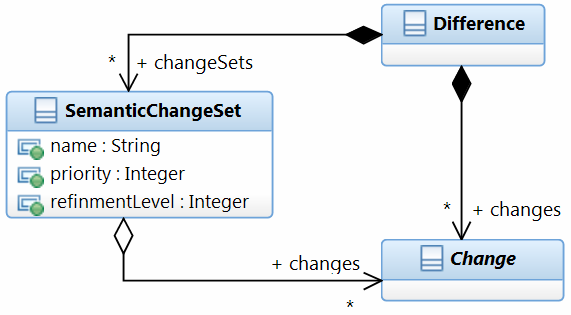
\includegraphics[scale=0.5]{images/semantic_change_set.png}
  \caption{Semantic-Change-Set}
  \label{fig:scs}
\end{figure}